\chapter{In-depth component description}

\section{Communicating with Channels}

\texttt{Channel} is an interface for performing I/O operations. It represents the principal abstraction used by the middleware to communicate with hardware devices and external software services.

The \texttt{Channel} interface is not tied to any specific technology or communication stack; as a result of this design choice, a wide variety of data management tasks, including but not limited to networking, file handling, and automatic data generation can be implemented as \texttt{Channel}s.

The current middleware architecture encourages the creation of several highly specialized \texttt{Channel}s, which are usually developed around third-party communication libraries. \texttt{HTTPChannel}, a \texttt{Channel} providing support for HTTP communications, is an excellent example of the advantages of this design strategy. Implemented as a simple wrapper around Apache's HTTP Components toolkit, its development only required a basic understanding of the HTTP protocol; yet \texttt{HTTPChannel} is a fully compliant HTTP/1.1 client (see section~\ref{sec:channel.implementations} for additional details).

Upon instantiation, \texttt{Channel}s are open and ready to be used. They may be optionally closed to relinquish unused resources by invoking the \texttt{close()} method. Once closed, a \texttt{Channel} cannot be re-opened, and every subsequent attempt to perform an I/O operation will fail causing a \texttt{ChannelException} to be thrown. The current state of a \texttt{Channel} can be probed through its \texttt{isClosed()} method.

\lstset{language=Java}
\begin{lstlisting}[float,floatplacement=H,caption=The Channel interface,label={lst:channel}]
public interface Channel {
	public String getId();
	
	public IOTask submit(IORequest request, IOHandler handler)
			throws ChannelException;
	
	public void setAsyncIOHandler(IOHandler handler)
			throws IllegalStateException;
			
	public boolean isClosed();
	
	public void close();		
}
\end{lstlisting}

All user-initiated I/O operations begin with an invocation of the \texttt{submit()} method. As can be seen in listing~\ref{lst:channel}, \texttt{submit()} is a direct implementation of the asynchronous interaction paradigm introduced in section~\ref{sec:newmiddleware.async}.

The emphasis on asynchronous execution is underscored by the absence of blocking operations in the \texttt{Channel} interface. This aspect is of paramount importance for the entire Middleware design, as implementing a truly asynchronous system would prove impossible if such feature were not provided by its core data access layer.


\section{Instantiating Channels}

Creation of new \texttt{Channel}s is performed by means of the  \texttt{ChannelFactory} interface, an actual reifications of the Factory design pattern that allows polymorphic instantiation of object classes.

By using the Factory instantiation model, the choice of a particular \texttt{Channel} implementation can be postponed from compile time to run time. This technique allows the Middleware to dynamically adapt in response to environment changes, and to support extension through the addition of new user-defined \texttt{Channel}s. For further information regarding the Factory pattern and its uses inside the PerLa Middleware, refer to section~\ref{sec:newmiddleware.factory}.

\lstset{language=Java}
\begin{lstlisting}[float,floatplacement=H,caption=The ChannelFactory interface,label={lst:channelFactory}]
public interface ChannelFactory {
	public Class<? extends ChannelDescriptor>
			acceptedChannelDescriptorClass();

	public Channel createChannel(ChannelDescriptor descriptor)
			throws InvalidDeviceDescriptorException;

}
\end{lstlisting}

All information required to create a new \texttt{Channel} instance must be stored inside a \texttt{ChannelDescriptor}. As shown in listing~\ref{lst:channelFactory}, this configuration object is the only parameter required to correctly invoke the \texttt{createChannel()} method.

Each \texttt{ChannelFactory} is tied to a specific communication technology; therefore, it can only accept a single class of \texttt{ChannelDescriptor} objects. For example, the \texttt{HTTPChannelFactory} parses \texttt{HTTPChannelDescriptor}s and creates \texttt{HTTPChannel}s, whereas the hypothetical \texttt{SerialChannelFactory} would parse \texttt{SerialChannelDescriptor}s to create \texttt{SerialChannel}s. Failure to provide a suitable \texttt{ChannelDescriptor} object will cause the \texttt{createChannel()} method to fail, throwing an \texttt{InvalidDeviceDescriptorException}.

\begin{figure}
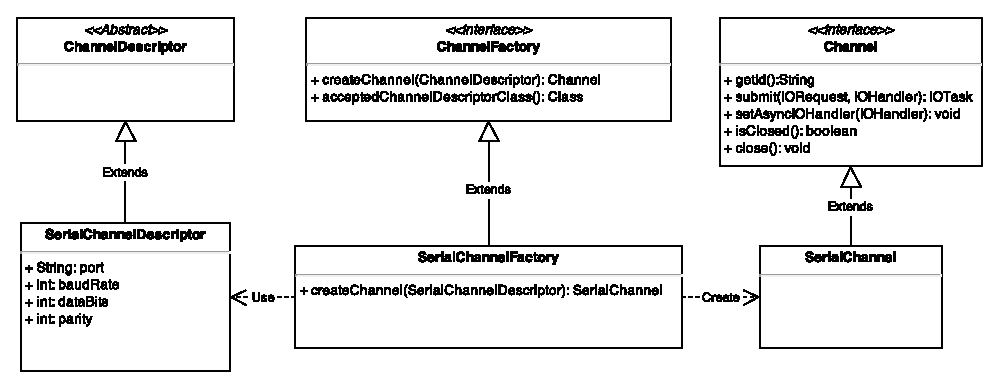
\includegraphics[width=\textwidth]{imgs/channel_factory.eps}
\caption{Class diagram of the Channel layer}
\end{figure}

The type of \texttt{ChannelDescriptor} accepted by a \texttt{ChannelFactory} can be queried with the \texttt{acceptedChannelDescriptorClass()} method. This dynamic discovery mechanism is the fulcrum of the Middleware plugin system, as it allows the \texttt{FPCFactory} to invoke the most appropriate \texttt{ChannelFactory} using only information available at runtime.

Contents of the \texttt{ChannelDescriptor} are loaded at runtime from an XML representation; this process is automatically performed by the JAXB library, which is also responsible for instantiating the correct \texttt{ChannelDescriptor} class using XML Namespace information (refer to section~\label{sec:newmiddleware.descriptor} for additional details).

Since the 



Previous design had a single channel, multiplexed through a channelmanager so tat it could be used by different fpc. Now there is a single channel instance for each fpc, and if multiplexing still has to be done, it has to be implemented by each single channel (maybe I wouldn't brag about this)


\subsection{IORequest management}

Every user-initiated interaction with a \texttt{Channel} begins with the creation of an appropriate \texttt{IORequest}, an object that contains all parameters required to characterize the I/O operation being started. Different \texttt{Channel}s require different \texttt{IORequest}s, since the parameters needed for starting an I/O operation depend upon the technical characteristics of the I/O operation itself.


Every \texttt{Channel} comes bundled with one or more \texttt{IORequest} concrete classes. \texttt{IORequest}s objects that are used to pass





\section{Performing I/O operations}


The outcome of an I/O operation are collected through the \texttt{IOHandler} passed as parameter to the \texttt{submit()} method. 

\texttt{submit()} requires the caller to specify an \texttt{IOHandler} callback object, through which data and errors will be notified once the requested operation is complete.

The execution of an ongoing I/O operations can be monitored and altered using the \texttt{IOTask} object returned 






Every user-initiated interaction with a \texttt{Channel} begins with the creation of an appropriate \texttt{IORequest}, an object that contains all parameters required to characterize the I/O operation being started. Different \texttt{Channel}s require different \texttt{IORequest}s, since the parameters needed for starting an I/O operation depend upon the technical characteristics of the I/O operation itself.

Since the specific contents of an \texttt{IORequest} object vary with the type of , the middleware does not provide a universal implementation for the \texttt{IORequest} object, 


A class of \texttt{IORequest} objects is tipically designed to be used with a specific \texttt{Channel} implementation, as its contents strictly depend on the gamut of operations supported by the \texttt{Channel} by which it is supposed to be executed 

The specific contents of an this object depend on the type of operations supported by the \texttt{Channel} that will perform

Different communication tasks require different parameters to be performed successfully: an appropriate URL is needed 

It is clear, even from this short lists of examples, that different IORequest objects

As such, a class of \texttt{IORequest} objects is typically...

 A class of \texttt{IORequest} objects is tipically designed to be used with a specific \texttt{Channel} implementation, as its contents strictly depend on the gamut of operations supported by the \texttt{Channel} by which it is supposed to be executed (e.g., \texttt{HTTPIORequests} can only be processed by an \texttt{HTTPChannel}). For this reason, the middleware does not provide a default implementation is provided for the \texttt{IORequest} interface. A set of guidelines for the implementation and management of \texttt{IORequest} objects will follow in the next sections of this chapter.

\texttt{IORequest} objects can be submitted to a \texttt{Channel} by means of the \texttt{submit()} method. As can be seen in listing~\ref{lst:channel}, this method is a direct implementation of the asynchronous invocation paradigm introduced in section~\ref{sec:newmiddleware.async}. Calls to \texttt{submit()} are non-blocking and require the caller to specify an \texttt{IOHandler} callback object, through which data and errors will be notified once the requested operation is complete.

The status of an ongoing operation can be queried and modified with the \texttt{IOTask} object, which is returned upon submitting a new request.


\lstset{language=Java}
\begin{lstlisting}[float,floatplacement=H,caption=The IOHandler interface,label={lst:iohandler}]
public interface IOHandler {
	public void complete(IORequest request, Optional<Payload> result);
	
	public void error(IORequest request, Throwable cause);
}
\end{lstlisting}

\lstset{language=Java}
\begin{lstlisting}[float,floatplacement=H,caption=The IOTask interface,label={lst:iotask}]
public interface IOTask {
	public void cancel();
	
	public IORequest getRequest();
	
	public boolean isCancelled();
	
	public boolean isDone();
}
\end{lstlisting}







There is no limit on the number of channels used by an FPC. Complex behaviours can be implemented using different channels

Interface description: methods, IORequest, IOHandler IOTask and Payload.
ByteArrayPayload description

The new Channel structure is monolithic, in that it contains all network layers required for the communication. This is in contrast with the previous middleware architecture, where communication layers where diveded between the legacy Channel implementation and the FPC. This new structure allows better reuse of off-the-shelf libraries.

ChannelFactory interface, methods and generic ChannelDescriptor structure

Basic XML 

IORequestBuilder and IORequestBuilderFactory

\subsection{Handling asynchronous data transmissions}

setAsyncIOHandler, how does it work and why do we need it

\subsection{Implementations: HTTPChannel and SimulatorChannel}
\label{sec:channel.implementations}

Full examples of actual implementations, complete with XML descriptor snippets


\section{Encoding and decoding information}

\subsection{The Message and Mapper interfaces}

\subsection{Handling composite data structures}

\subsection{Managing multiple message types}

\subsection{Implementations: JSONMapper and URLEncodedMapper}


\section{Data management: Scripts}

\subsection{From Messages to Records}

\subsection{Available instructions}

\subsection{Engine architecture and execution model}

\subsection{Script examples}


\section{Putting it all together: the FPC}

\subsection{Data access interface}

\subsection{Controlling the remote device}

\subsection{Scheduling mechanism}


\section{Device Descriptor and FPC Factory}

\subsection{The XML Device Descriptor}

\subsection{FPC Factory}

\subsection{Registry}

\subsection{Complete XML Device Descriptor examples}